\section{Motivace a myšlenka experimentu}

Jedním z nástrojem ke zkoumání vlastností broušeného kamene je nasvícení jeho povrchu světelným svazkem. Na fasetách broušeného kamene dochází ve zjednodušeném případě k odrazu a lomu světelného svazku. Z toho důvodu se dopadající světelný svazek roztříští na řadu světelných svazků, které z kamene vystupují v různých směrech, s rozdílným zářivým tokem a dalšími typickými vlastnostmi, jako je například polarizace. 
Vystupující světelné svazky lze zachytit na stínítku. Obrazec vzniklý na stínítku jednoznačně charakterizuje broušený kámen. 

Pro tento experiment nasvícení kamene již vznikla řada programů obsahující více či méně věrohodný matematický model. Máme tedy možnost průlet světelného svazku kamenem simulovat. 

V našem případě využíváme program LADOK, který vznikl v Centru strojového vnímání na katedře Kybernetiky ČVUT v Praze. Simulační program LADOK dostatečně přesně určuje matematický model experimentu.

Cestou, jak určit tvar a další typické vlastností kamene, je rozpoznat vystupující paprsky a nalézt takový matematický model, jehož výstup by odpovídal reálné situaci (obrazci na stínítku). 

Problém však tkví v rozpoznání světelných svazků. V tomto případě jde o to ke každému svazku, viditelném na stínítku, přiřadit správnou posloupnost faset kamene, přes které se světelný svazek lomil nebo odrážel. Parametry svazku, které nám pomáhají rozpoznat jeho cestu jsou směr (azimut, elevace), zářivý tok, intenzita, plocha, velikost a směr světelných šmouh, dále nazývaných ocásky, vznikajících při průchodu světelného svazku přes hranu kamene. 

Cílem experimentu je pokusit se nalézt další parametr světelného svazku, jenž by v kombinaci s ostatními parametry pomohl svazek správně rozpoznat. 

Pokusíme se naleznout směr či velikost posunu světelných svazků při rotaci kamene nebo při naklonění zdroje dopadajícího světelného svazku. 

\newpage
\section{Popis problému}

Rotace kamene kolem osy způsobí změnu vlastností vystupujících světelných svazků (směru, zářivého toku, intenzity, vlastnosti ocásků atd.). Za určitých okolností může světelný svazek zcela vymizet. Tato situace nastává například při lomu světelného svazku z kamene do okolí. Když vlivem rotace překročíme kritický úhel, nedochází k vylomení světelného svazku, ale k totálnímu odrazu na fasetě. Světelný svazek také postupně zmizí při posunu světelného svazku mimo fasetu, a to jak při odrazu, tak při lomu. Ze stejných důvodů, proč mohou světelné svazky vymizet, mohou naopak vzniknout svazky nové.

Uvažujeme zjednodušenou situaci. Světelný svazek nahradíme světelným paprskem ležícím v jeho pomyslném těžišti. 

Světelný paprsek necháme dopadat na zrcadlo pod úhlem $\varphi_1$ a od nějž se odráží podle známého zákonu odrazu pod úhlem $\varphi_1$. Při vychýlení světelného paprsku o úhel $ \delta $ v kladném směru úhlu $\varphi_1$ je odražený úhel $\varphi_1 + \delta$. Odražený paprsek se otočí o úhel $ \delta $.

\begin{figure}[h!]
\begin{center}
\scalebox{1}{ \input{xfig/odraz2.pstex_t}}
\end{center}
\caption{Odraz laseru od zrcadla. Změna úhlu dopadajícího světelného paprsku vyvolá stejně velkou změnu úhlu odraženého paprsku.}
\label{fig:odraz laser}
\end{figure}

Jiná situace nastává při rotaci zrcadla kolem osy o úhel $\alpha$ v záporném směru. Světelný paprsek dopadá na zrcadlo pod úhlem $\varphi_1 + \alpha$. Odráží se pod úhlem $\varphi_1+\alpha$, ale vzhledem k tomu, že vstupní parsek je ve stejné pozici, se výstupní paprsek otočí o úhel  $2\alpha$. 


Důsledkem toho dostaneme identické výsledky experimentu při rotaci kamene, jako při natočení světelného zdroje o dvojnásobný úhel v opačném směru. Dále budeme tedy uvažovat pouze rotaci kamene. 

\newpage
\begin{figure}[h!]
\begin{center}
\scalebox{1}{ \input{xfig/odraz.pstex_t}}
\end{center}
\caption{Odraz laseru od rotujícího zrcadla. Rotace zrcadla vyvolá dvojnásobnou změnu velikosti úhlu odraženého paprsku.}
\label{fig:odraz zrcadlo}
\end{figure}

Pokud by docházelo pouze k odrážení od zrcadel v dvojrozměrné rovině, tak by naše zkoumání postrádalo smysl. Výstupní parsek by se vždy otočil o dvojnásobek úhlu rotace kamene, a to ve stejném směru. 

S uvažováním materiálu kamene s konstantním indexem lomu $ n_1>1 $ a okolí s indexem lomu $ n_2 = 1 $ se situace dramaticky mění. Vezměme si příklad lomu světelného paprsku z kamene přes rovinnou fasetu. Úhel dopadajícího paprsku na fasetu označme $\alpha_1$ a úhel lomeného svazku $\alpha_2$, pak můžeme podle Snellova zákonu psát:

\begin{center}
$n_1\,\sin(\alpha_1) = n_2\,\sin(\alpha_2) = \sin(\alpha_2)\,.$
\end{center}

\begin{figure}[h!]
\begin{center}
\scalebox{.9}{ \input{xfig/index.pstex_t}}
\end{center}
\caption{Tři případy, které mohou nastat při dopadu světelného paprsku na fasetu. Zleva lom paprsku z kamene, dopad pod kritickým úhlem a totální odraz.}
\label{fig:lom ven }
\end{figure}

Zkoumejme změnu výstupního úhlu $\alpha_2$ na změně úhlu $\alpha_1$. Nejprve si vyjádříme úhel $\alpha_2$ následně zderivujeme podle $\alpha_1$. 
\begin{eqnarray}
\alpha_2 = \arcsin(n_1\,\sin\alpha_1) \implies \frac{\mathrm{d}\alpha_2}{\mathrm{d}\alpha_1}= \frac{n_1\,\cos\alpha_1}{\sqrt{1-n_1^2\,\sin^2\alpha_1}}\,.
\label{eq:derivace uhlu}  
\end{eqnarray}

Pokud se dostáváme ke kritickému úhlu $\alpha_k$, kdy dochází k totálnímu odrazu, potom
\begin{center}
 $	\sin\alpha_2 = 1 \implies \sin\alpha_1 = \frac{1}{n_1}\,. $
\end{center}

Změnu výstupního úhlu $\alpha_2$ a vypočtením limity v okolí kritického úhlu pro $ n_1>1$ dostaneme 

\begin{eqnarray}
\lim_{n \to \alpha_k}\frac{\mathrm{d}\alpha_2}{\mathrm{d}\alpha_1} = \frac{n_1\,\cos(\arcsin\frac{1}{n_1})}{\sqrt{1-n_1^2\,\frac{1}{n_1^2}}} \to \infty\,.
\label{eq:zmena velikosti posunu}  
\end{eqnarray}
Z grafu \ref{fig:derivace uhlu} zjistíme, že minimum funkce $\frac{\mathrm{d}\alpha_2}{\mathrm{d}\alpha_1}$ vychází pro $ \alpha_1 = 0^\circ $. Po dosazení
\begin{eqnarray}
{\frac{\mathrm{d}\alpha_2}{\mathrm{d}\alpha_1}}\biggr\rvert_{\alpha_1 = 0^\circ}= \frac{n_1}{\sqrt{1-0}} = n_1\,.
\end{eqnarray}


Velikost změny posunu světelného svazku tedy může být teoreticky libovolně větší než je index lomu $n_1$. 

\begin{figure}[h!]
\begin{center}
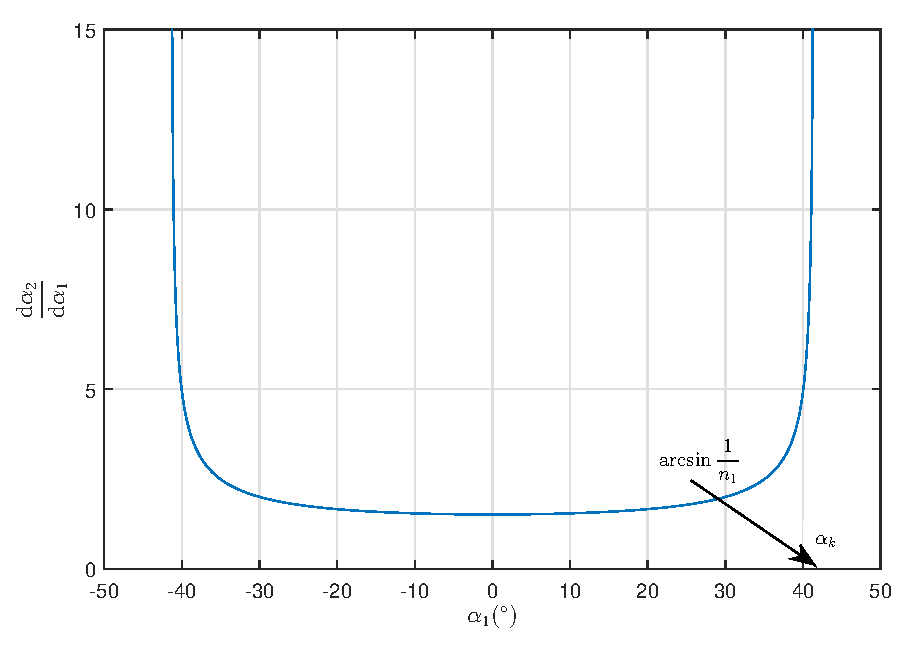
\includegraphics[width = 8cm]{figures/derivace.eps}
\end{center}
\caption{Závislost změny lomeného úhlu na velikosti dopadajícím úhlu. Pro kritický úhel roste k nekonečnu. Graf funkce popsané vzorcem \ref{eq:zmena velikosti posunu}.}
\label{fig:derivace uhlu}
\end{figure}
\newpage


\section{Modelování pohybu světelných svazků v programu LADOKU}

V programu pro simulaci průchodu světelného paprsku konvexním objektem jsme provedli experiment s rotací broušeného kamene. Pro svoji jednoduchost jsme vybrali kámen ve tvaru šatonové růže s 12 bočními fasetami, tabulkou a spodkem ideálního tvaru (VIVA12).

Rotací kamene okolo osy kolmé ke spodku kamene dostaneme pouze soustředné kružnice. Kámen jsme tedy rotovali kolem vodorovné osy procházející středem spodku kamene o konstantní úhel v každém kroku. Zaznamenali jsme směry vystupujících svazků při různých pozicích kamene. Výsledek jsme vykreslili do polárního grafu. Ze dvou po sobě následujících pozic kamene jsme šipkou spojili pozici svazků se stejnou historií odrazu a lomů od faset kamene. Výsledný obrazec je znázorněn a grafu \ref{fig:relativni pohyb graf}.

Z praktického hlediska nás potom mohou pouze svazky, jejichž stopy lze na stínítku detekovat.

% obrazek pohybu jednotlivych stop 
\begin{figure}[h!]
\begin{center}
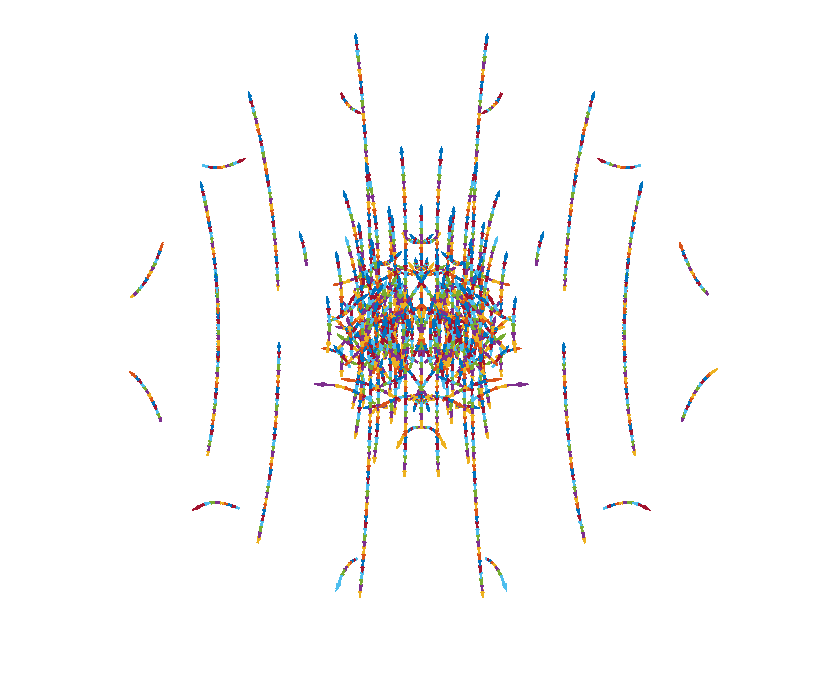
\includegraphics[width = 10cm]{figures/viva12_bigflux.eps}
\end{center}
\caption{Dráhy jednotlivých světelných stop svazků vycházejících z kamene VIVA12 získané pomocí simulačního programu  LADOK. Zobrazeny jsou pouze svazky s významnou energií vycházející v horního poloprostoru kamene. }

\label{fig:relativni pohyb graf}
\end{figure}

\newpage
Pro lepší představu o změně natočení jednotlivých svazků nám může být užitečný kruhový histogram znázorňující směr jejich pohybu (obr. \ref{fig:relativni pohyb graf}). Na něm vidíme, že větší část se pohybuje ve směru rotace kamene. Podstatná většina svazků se posouvá ve směru rotace kamene, což ovšem není příliš nápomocné při jejich identifikaci.

Existují však svazky, které jsou svým pohybem charakteristické a lze je tedy oddělit od ostatních. Kritériem pro rozpoznání svazků nemusí být pouze směr pohybu, ale jak vidíme na obr. \ref{fig:relativni pohyb graf} i velikost. V neposlední řadě přichází v úvahu i změna zářivého toku svazků, změna velikosti ocásků a další. 

\begin{figure}[h!]
 \begin{center}
 

   \begin{minipage}[c]{0.45\textwidth}
     \centering 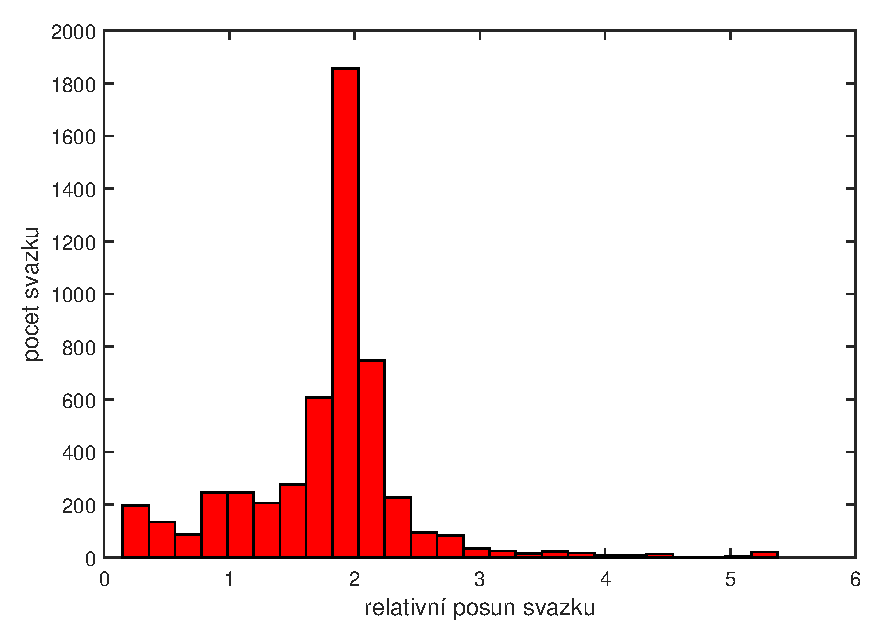
\includegraphics[height =4.5cm]{figures/relative.eps} 
   \end{minipage}
   \begin{minipage}[c]{0.45\textwidth}
     \centering 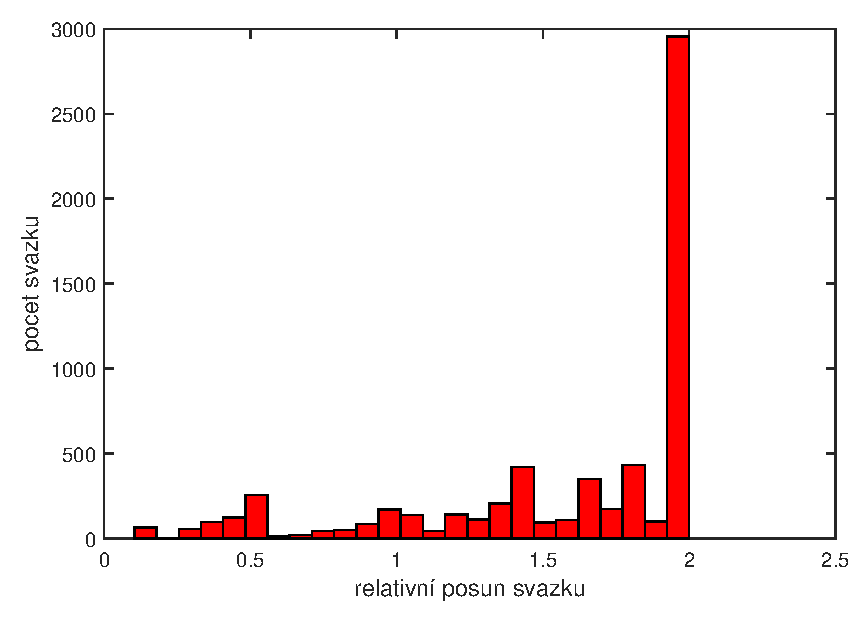
\includegraphics[height =4.5cm]{figures/relative_index1.eps} 
   \end{minipage}
 \end{center}
\caption{Vlevo histogram velikosti natočení světelných svazků kamene VIVA12 z obrázku \ref{fig:relativni pohyb graf}. Vlivem lomu je relativní natočení v mnoha případech vetší než 2. V okolí kritického úhlu roste změna k nekonečnu. Pokud ztotožníme indexy lomu kamene a okolí, tak relativní natočení nebude větší než 2. To lze vidět na histogramu vpravo.}

\label{fig:histogram relativni pohyb }

\end{figure}

Vykresleme si histogram (obr. \ref{fig:histogram relativni pohyb } vlevo) relativní velikosti natočení vystupujících svazků. Z něj je patrné, že řada svazků rotuje o více než dvojnásobek úhlu rotace kamene $\alpha$, což potvrzuje teorii o relativní změně velikosti natočení z rovnice \ref{eq:zmena velikosti posunu}. 



\begin{figure}[h!]
\begin{center}
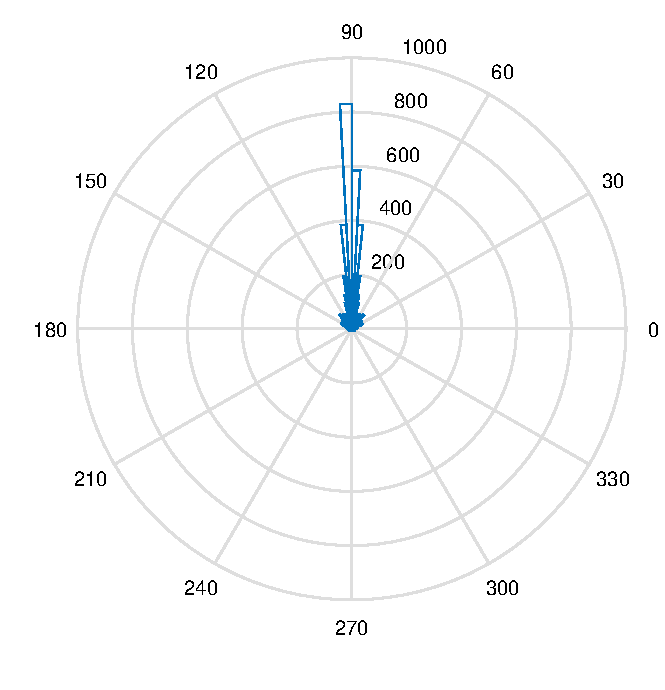
\includegraphics[width = 7cm]{figures/kruhovy_histogram.eps}
\end{center}
\caption{Kruhový histogram směru pohybu jednotlivých světelných svazků kamene VIVA12 z obrázku \ref{fig:relativni pohyb graf}. Většina stop se pohybuje ve směru rotace kamene.}
\label{fig:kruhovy histogram}
\end{figure}

Pokud vezmeme teoreticky kámen o stejném indexu lomu, jako je okolí, neměl by se v kameni lom objevovat. Potom by se velikost rotace výstupního svazku úhel větší než $2\alpha$, způsobená právě rozdílným indexem lomu,  neměla vůbec objevovat. Pro potvrzení této teorie jsme provedli stejnou simulaci jako v předchozím případě. Indexy lomu kamene a jeho okolí jsme ztotožnili a výsledek simulace ukázal, že rotace výstupních svazků úhel větší než $2\alpha$ se již nevyskytují. To nám dokládá zhotovený histogram (obr. \ref{fig:histogram relativni pohyb } vpravo).


\begin{figure}[h!]
\begin{center}
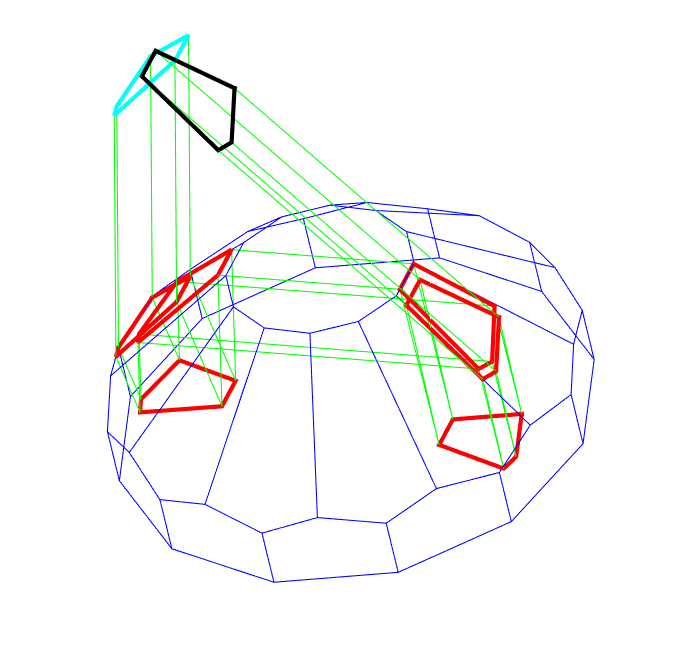
\includegraphics[width = 7cm]{figures/odraz.eps}
\end{center}
\caption{Průlet světelného svazku kamenem VIVA12. Příklad s velkou změnou vystupujícího úhlu. Dopad světelného svazku na fasetu kamene je znázorněn hranolem s modrým okrajem. Svazek vystupující z kamene je hranol s černým okrajem. Svazek kamenem putuje následovně: 1. lom do kamene, 2. odraz od spodku, 3. odraz od fasety, 4. odraz od fasety na protější straně, 5. odraz od spodku, 6. dopad na fasetu pod úhlem blízkým kritickému úhlu a lom z kamene.}

\label{fig:odrazy v kamenu}
\end{figure}
\newpage

Téměř konstantní směrovost rotace svazků u kamene VIVA12 zmenšuje význam příspěvku této vlastnosti k lepšímu rozpoznání světelných stop. Pokud ovšem provedeme stejný experiment na broušeném kameni jiného tvaru, dostaneme rozdílný výsledek. Například u šatonu, svým tvarem složitějším než VIVA12, je směr rotace svazků rozmanitější. Velká část z nich samozřejmě rotuje ve směru rotace kamene. Jak ale vidíme z kruhového histogramu (obr. \ref{fig:kruhovy histogram saton}), lze rozlišovat i velké množství stop pohybujících se např. pod úhlem $45^\circ$. U šatonu tedy může směr pohybu svazků nemalou měrou pomoci v jejich rozpoznání. 

\begin{figure}[h!]
\begin{center}
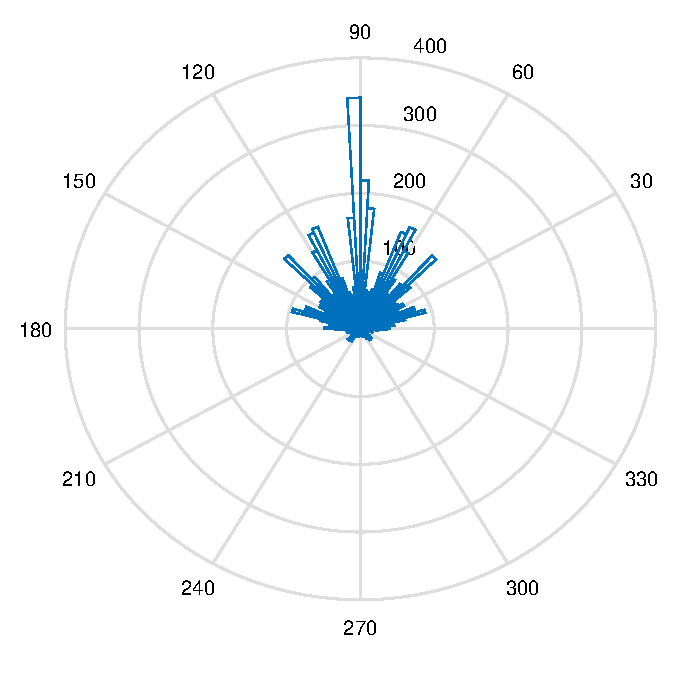
\includegraphics[width = 7cm]{figures/saton_smer.eps}
\end{center}
\caption{Kruhový histogram směru rotace jednotlivých světelných svazků u šatonu. Svazky se natáčí různými směry, kterými lze svazky charakterizovat.}

\label{fig:kruhovy histogram saton}
\end{figure}

  
%\clearpage